\documentclass{lab1-article}

\title{Indice di rifrazione e focale di una lente}

\input{python}

\begin{document}


\begin{article}
\selectlanguage{italian}

\maketitle

\secsummary

L'obiettivo dell'esperienza consiste nella misura dell'indice di rifrazione
del plexiglass e dellla lunghezza focale di una lente divergente.


\secmaterials

\begin{itemize}
\item Banco ottico con sorgente luminosa;
\item un semicilindro di plexiglass;
\item una cassetta di lenti;
\item un supporto per il plexiglass;
\item un metro a nastro (risoluzione $1$~mm).
\end{itemize}


\secmeasurements


\labsubsection{Indice di rifrazione del plexiglass}

\begin{figure}[htb!]
  \begin{tikzpicture}[scale=1]
    \pgfmathsetmacro{\xc}{4.5}
    \pgfmathsetmacro{\yc}{0}
    \pgfmathsetmacro{\r}{2.25}
    \pgfmathsetmacro{\rthetaa}{0.7}
    \pgfmathsetmacro{\rthetab}{0.75}
    \pgfmathsetmacro{\l}{4}
    \pgfmathsetmacro{\thetain}{30}
    \pgfmathsetmacro{\thetarif}{20}
    \node at (0, 0) {};
    \draw (\xc, \yc) arc (90:270:\r);
    \draw (\xc, \yc)--(\xc, \yc-2*\r);
    \draw[style=densely dashed] (0, \yc - \r)--(8, \yc - \r);
    \draw (\xc, \yc-\r)--(\xc+\l*cos{\thetain}, \yc-\r+\l*sin{\thetain});
    \draw (\xc, \yc-\r)--(\xc-\l*cos{\thetarif}, \yc-\r-\l*sin{\thetarif});
    \draw (\xc+\rthetaa, \yc-\r) arc (0:\thetain:\rthetaa);
    \draw (\xc+\rthetab, \yc-\r) arc (0:\thetain:\rthetab);
    \draw (\xc-\rthetab, \yc-\r) arc (180:180+\thetarif:\rthetab);
    \node at (\xc+2*\rthetab*cos{\thetain},%
    \yc-\r+2*\rthetab*sin{\thetain/2}) {$\theta_{\rm i}$};
    \node at (\xc-2*\rthetab*cos{\thetarif},%
    \yc-\r-2*\rthetab*sin{\thetarif/2}) {$\theta_{\rm r}$};
    \node at (\xc+2*\rthetaa, \yc-1.5*\r) {$n_1 \sim 1$};
    \node at (\xc-1.25*\rthetaa, \yc-1.5*\r) {$n_2$};
  \end{tikzpicture}
  \caption{Schematizzazione dell'apparato per la misura dell'indice di
    rifrazione del plexiglass.
    L'angolo di incidenza $\theta_{\rm i}$ (di rifrazione $\theta_{\rm r}$)
    \`e l'angolo formato dal raggio luminoso incidente (rifratto) con la
    normale alla superficie di separazione tra i due mezzi.}
  \label{fig:plexiglass}
\end{figure}


Se un raggio di luce passa da un mezzo con indice di rifrazione $n_1$ ad
uno con indice di rifrazione $n_2$, gli angoli di incidenza e di rifrazione
sono legati tra di loro dalla legge di Snell
\begin{align}
  n_1 \sin\theta_{\rm i} = n_2\sin\theta_{\rm r}.
\end{align}

Si posizioni il semicilindro in modo che il raggio incida al centro della
superficie piana rifrangente (per evitare una seconda rifrazione in uscita) e
si misuri una serie di coppie $(\sin\theta_{\rm i},~\sin\theta_{\rm r})$ per un
certo numero (diciamo $10$) di valori di $\theta_{\rm i}$.
Si ricavi l'indice di rifrazione cercato da un fit lineare alle misure,
ricordando che l'indice di rifrazione dell'aria \`e con buona approssimazione
$n_1 \sim 1$.


\labsubsection{Lente divergente}

Dato che la lente divergente non forma immagini reali, per questa misura
occorre anche una lente convergente \emph{di potere diottrico maggiore (in
modulo) rispetto a quello della divergente}. Possiamo considerare l'immagine
prodotta dalla lente convergente come una sorgente virtuale per la lente
divergente.

\begin{figure}[htb!]
\begin{center}
  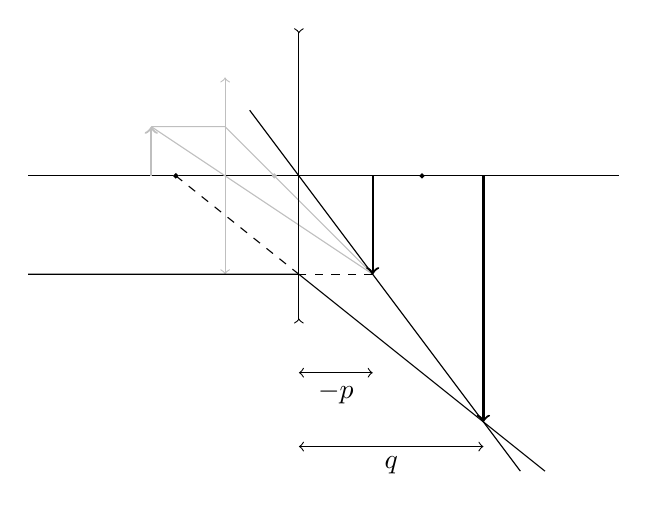
\begin{tikzpicture}[scale=1.25]
    %\draw (0, 0) -- (1,1);
    \draw (0, 0) -- (6,0);
    \draw[lightgray, ->] (2, 0) -- (2,1);
    \draw[lightgray,->] (2, 0) -- (2,-1);
    \draw [lightgray, fill] (1.5,0) circle [radius=0.02];
    \draw [lightgray, fill] (2.5,0) circle [radius=0.02];
    \draw[lightgray, thick, ->] (1.25, 0) -- (1.25,0.5); % old object
    \draw[lightgray] (1.25,0.5) -- (2, 0.5) -- (3.5, -1);
    \draw[lightgray] (1.25,0.5) -- (3.5, -1);
    \draw[thick, ->] (3.5, 0) -- (3.5,-1); % object (old image)
    % lens
    \draw[-<] (2.75, 0) -- (2.75,1.5);
    \draw[-<] (2.75, 0) -- (2.75,-1.5);
    \draw [fill] (4,0) circle [radius=0.02];
    \draw [fill] (1.5,0) circle [radius=0.02];
    % ray
    \draw[dashed] (3.5,-1) -- (2.75, -1);
    \draw[dashed] (2.75,-1) -- (1.5, 0);
    \draw (0,-1) -- (2.75, -1) -- (5.25, -3);
    \draw (2.25, 2./3) -- (5., -3);
    \draw[thick, ->] (15./8+2.75, 0) -- (15./8+2.75,-2.5); % image
    % notation
    \draw[<->] (2.75, -2.) -- (3.5, -2.);
    \node [below] at (3.125,-2.) {$-p$};
    \draw[<->] (2.75, -2.75) -- (15./8+2.75,-2.75);
    \node [below] at (3.69,-2.75) {$q$};

  \end{tikzpicture}
  \caption{Schema ottico per la lente divergente.
    Notare che la sorgente per la lente divergente \`e virtuale.}
  \label{fig:divergente}
\end{center}
\end{figure}

In pratica: si ponga la lente convergente sul banco ottico e si metta a fuoco
l'immagine sullo schermo. A questo punto si posizioni la lente divergente
tra la convergente e lo schermo e si misuri la distanza $p_i$ (da prendere con
il segno negativo) tra la divergente e lo schermo stesso. Si allontani lo
schermo in modo da rimettere a fuoco l'immagine e si misuri la nuova distanza
$q_i$ (questa volta positiva) tra la divergente e lo schermo. Come nel caso
precedente, si iteri il procedimento pi\`u volte (ad esempio 10) e si stimi
il potere diottrico tramite un \emph{fit} lineare.


\secconsiderations

\labsubsection{Indice di rifrazione del plexiglass}

Troverete gi\`a montati sul banco ottico, accanto alla sorgente di luce, una
lente convergente ed un diaframma a fenditura per creare un fascio di luce
sottile. Non dovrebbe essere necessario modificare il montaggio---in caso di
bisogno chiedete aiuto all'esercitatore.


\labsubsection{Focale della lente}

Quando si misura la distanza tra una lente ed una sorgente, potrebbe non essere
sufficiente prendere come errore la risoluzione del metro a nastro, in quanto
la posizione della lente nella ghiera di montaggio non \`e ben definita.
In altre parole la lente non \`e molto pi\`u sottile (e nemmeno pi\`u sottile)
della risoluzione del metro a nastro.

Quando si misura la distanza tra la lente e l'immagine, il contributo maggiore
all'errore di misura potrebbe essere dovuto alla messa a fuoco.


\end{article}
\end{document}
